\section{Architecture}
Die Architektur des Frameworks lässt sich mit einer mehrstufigen Pipeline, wie im unteren Teil von Abbildung \ref{fig:pipeline} zu sehen, vergleichen. Dabei können einzelne Komponenten ausgetauscht bzw. über die \textit{Meta tool chain} (siehe Abbildung \ref{fig:pipeline}, oberer Teil) konfiguriert werden.

\begin{figure}[h!]
\centering
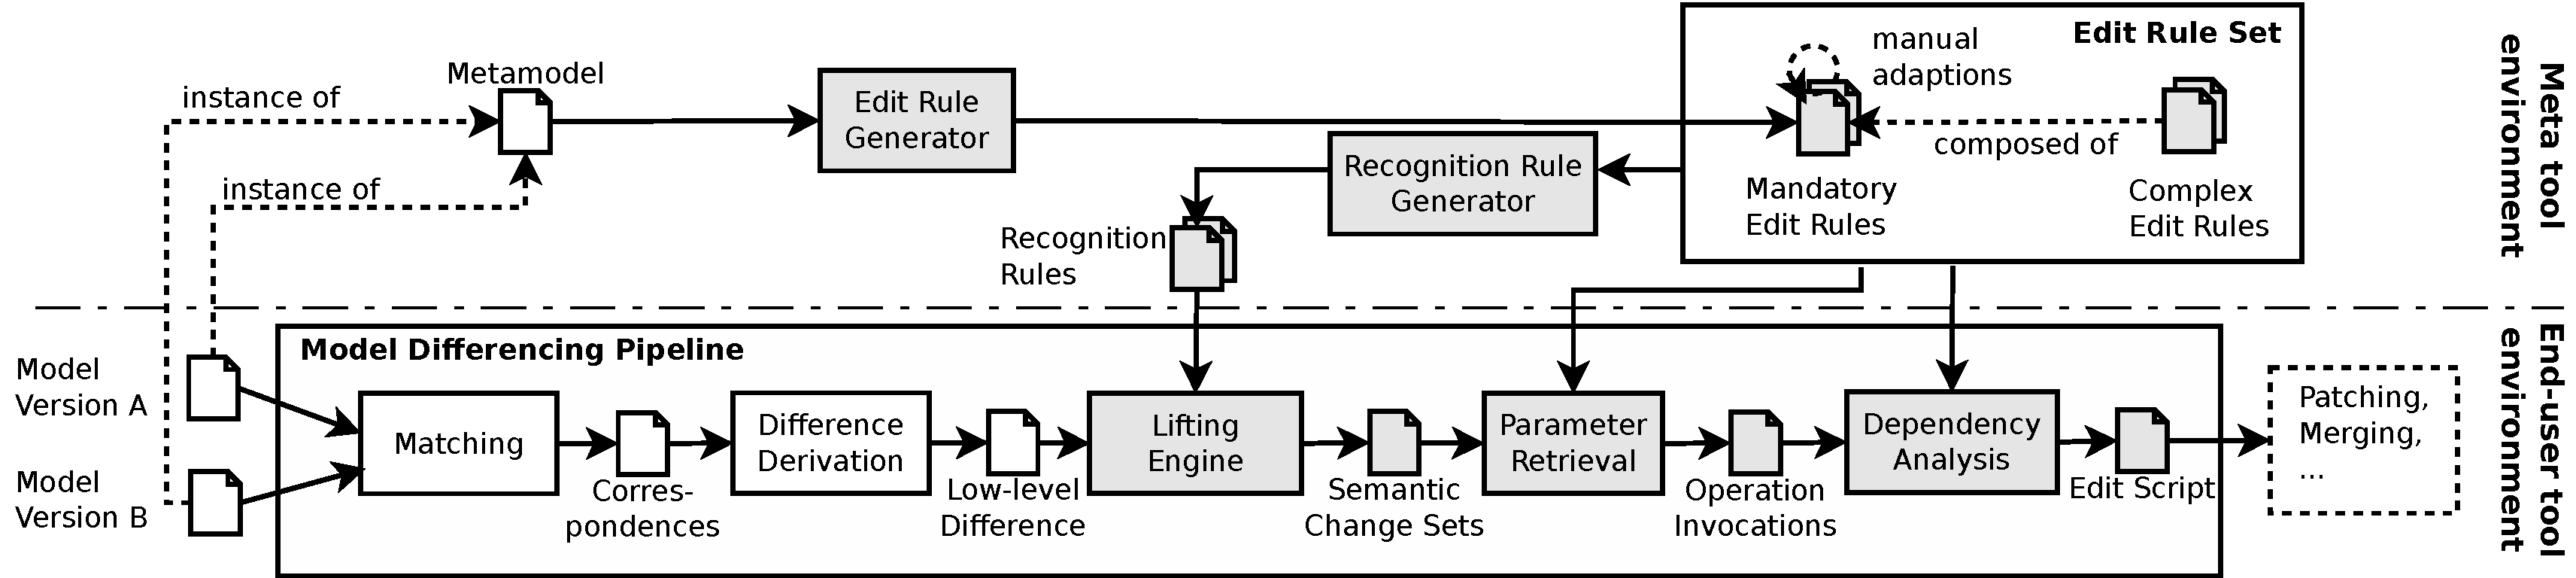
\includegraphics[width=\textwidth]{images/architecture/pipeline}
\caption{Differencing tool chain and meta-tools}
\label{fig:pipeline}
\end{figure}

Im folgenden werden die einzelnen Komponenten genauer erläutert.

\subsection{Matching}

Die Aufgabe des \textit{Matchers} ist es, die korrespondierenden Elemente aus Modell A und Modell B, also die Elemente, die in beiden Modellen übereinstimmen, zu identifizieren.
Dabei ist das Ergebnis vor allem davon abhängig anhand welcher Kriterien der Matcher eine Übereinstimmung festlegt.
Hier wird unter anderem zwischen \textit{ID-}, \textit{signatur-} und \textit{ähnlichkeitsbasierten} Verfahren unterschieden.\\
Das Framework definiert einen Extension Point (siehe \ref{exp:org.sidiff.matcher.extensionpoint}), welcher es ermöglicht weiter Matcher in das Framework zu integrieren.
Die konzeptuelle Struktur des Ergebnisses, also eines \textit{Matchings}, ist dabei durch das in Abbildung \ref{fig:matching_model} dargestellte, EMF-basierte Metamodell definiert.

\begin{figure}[h!]
\centering
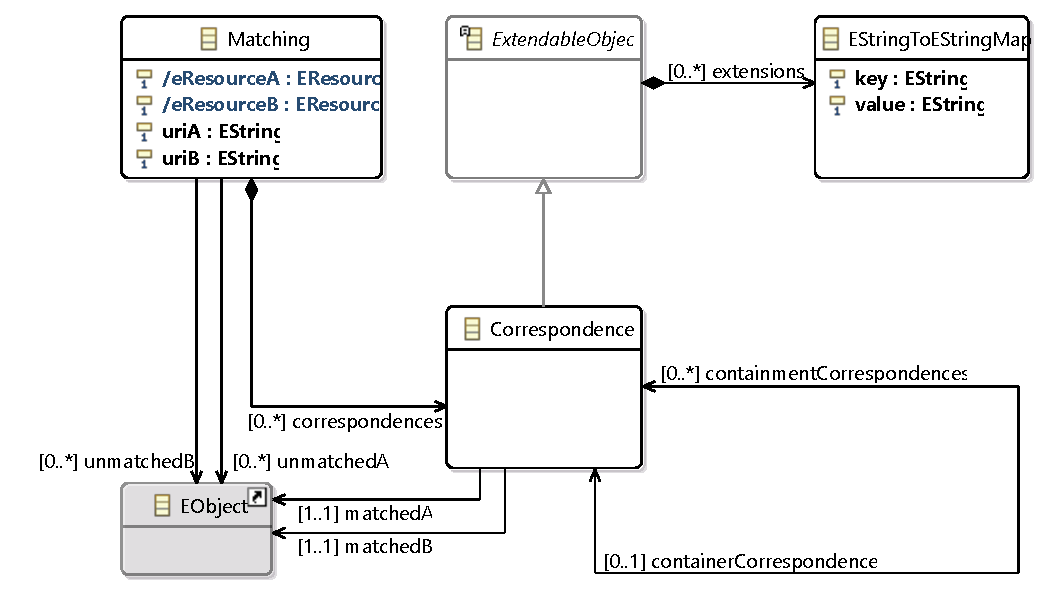
\includegraphics[width=0.75\textwidth]{images/architecture/matching_model}
\caption{Abstract Syntax of a model matching}
\label{fig:matching_model}
\end{figure}

Ein \texttt{Matching} zwischen den beiden Modellen \texttt{eResourceA} und \texttt{eResourceB} besteht aus einer Menge von \texttt{Correspondences}. Eine \texttt{Correspondence} verweist auf die beiden korrespondierenden Elemente \texttt{matchedA} und \texttt{matchedB} vom Typ \texttt{EObject}. Zusätzlich kann diese Referenzen auf die \texttt{Correspondence} der Kind- (\texttt{containmentCorrespondences}) bzw. der Elternelemente (\texttt{con\-tnai\-ner\-Correspondence}) halten.
Des Weiteren erbt eine \texttt{Cor\-res\-pon\-dence} von \texttt{ExtendableObject}, wodurch es möglich ist dieser weitere Eigenschaften, wie beispielsweise der Verlässlichkeit, zuzuordnen.\\

\newpage


\subsection{Difference Derivation}
Ausgehend von den gefunden Korrespondenzen berechnet der \textit{Difference Derivator} eine technische Differenz (\textit{low-level difference}) der Mo\-del\-le.
Alle Objekte und Referenzen, für die keine Korrespondenz existiert, müssen demnach entweder in Modell B hinzugefügt, oder aus Modell A entfernt worden sein. 
Durch die Verwendung eines \textit{Technical Difference Builders} können Modellelemente von der Differenzberechnung ausgeschlossen werden.
Dieser kann ebenfalls über einen Extension Point (siehe \ref{exp:org.sidiff.difference.technical.extensionpoint}) erweitert und für die jeweilige Domäne angepasst werden.\\
Die konzeptuelle Struktur einer Differenz ist durch das in Abbildung \ref{fig:technical_model} dargestellte, EMF-basierte Metamodell definiert. 

\begin{figure}[h!]
\centering
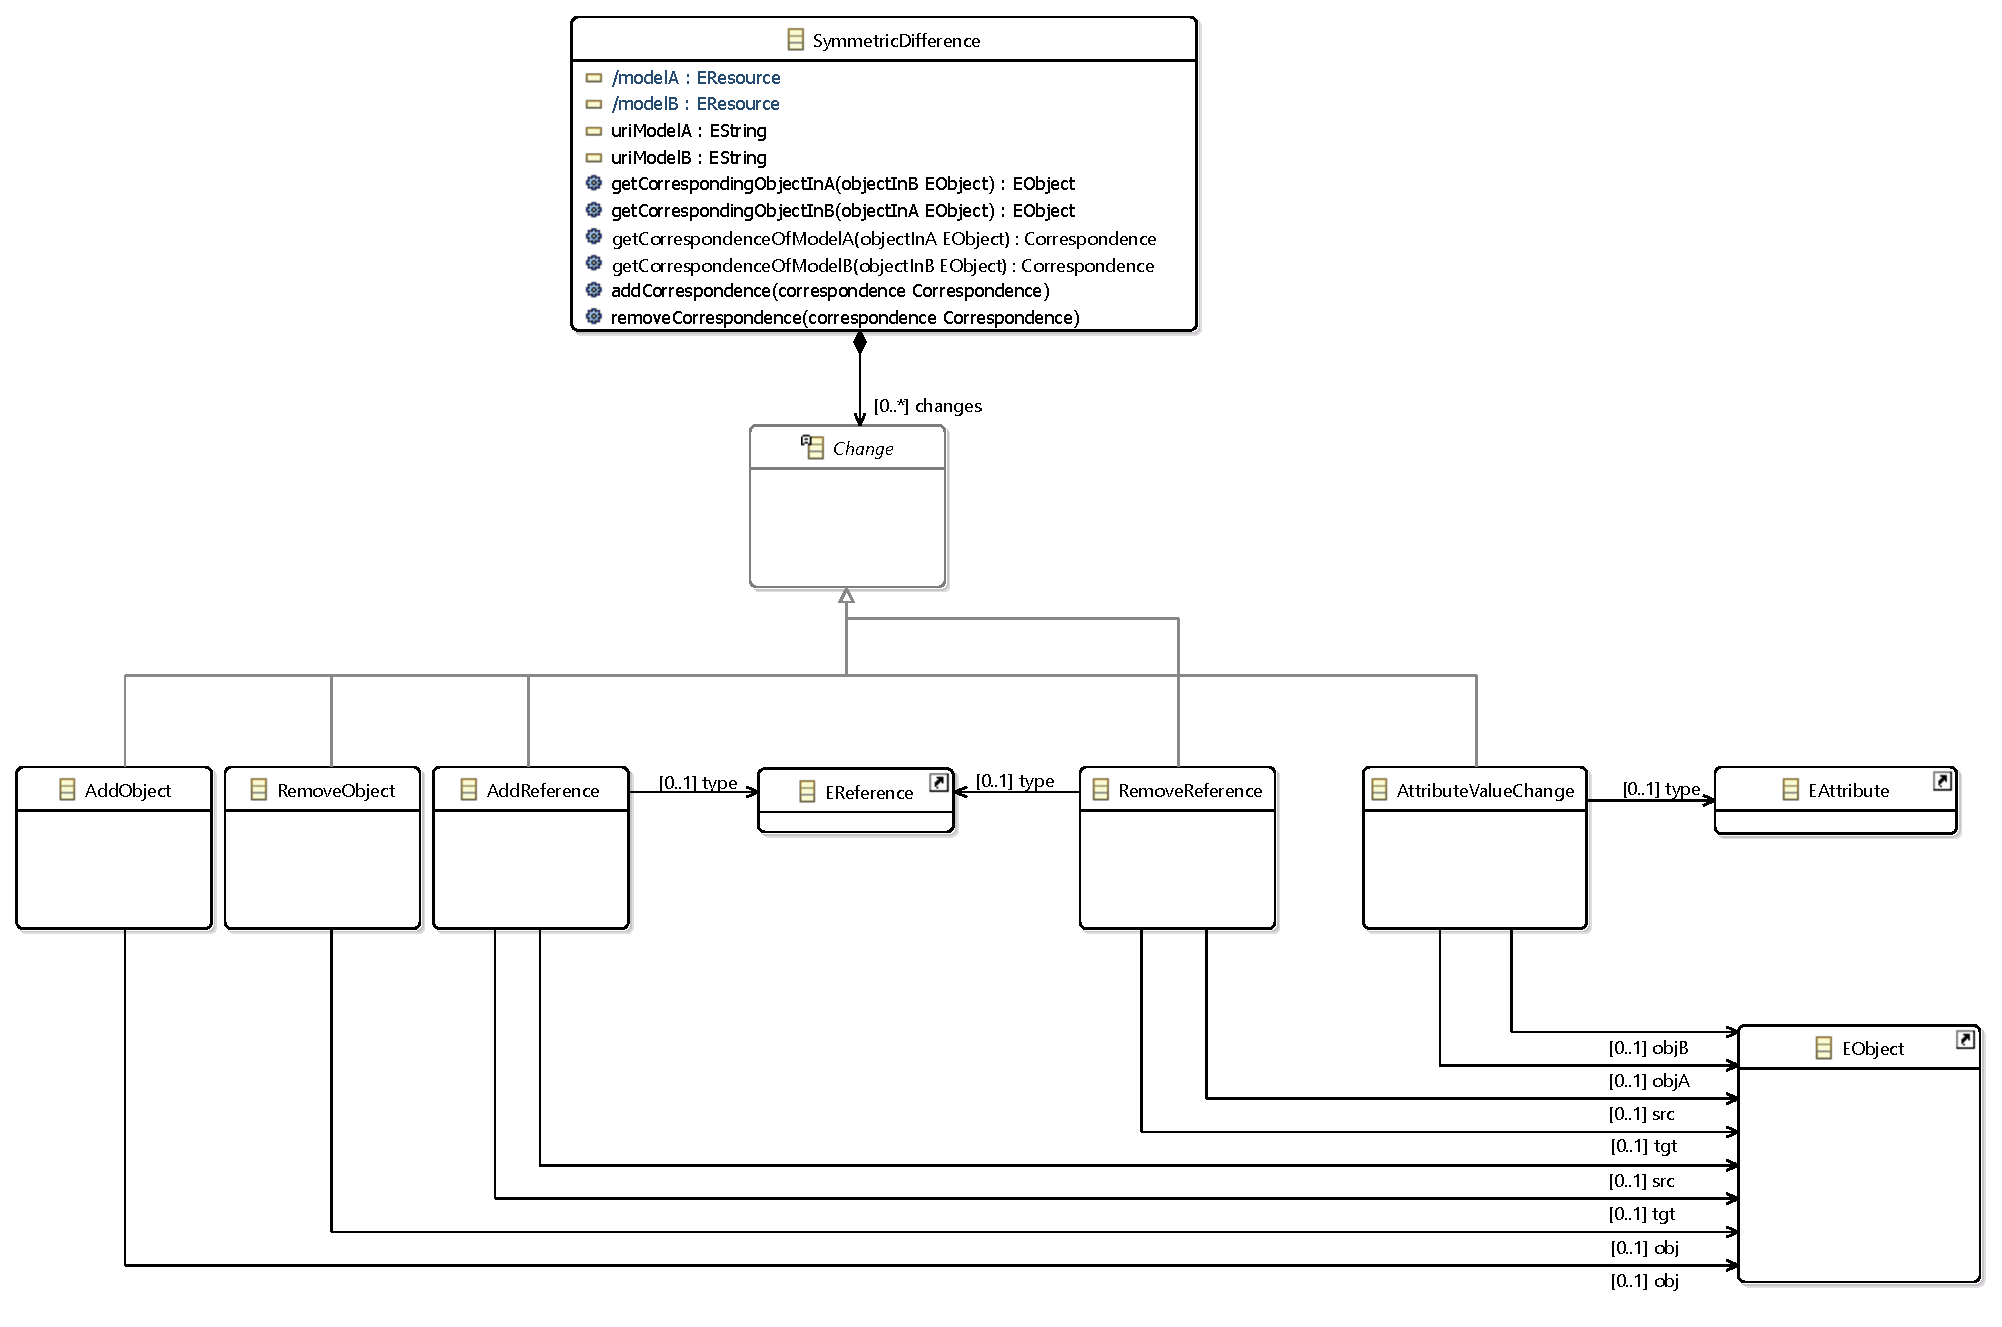
\includegraphics[width=\textwidth]{images/architecture/technical_model}
\caption{Abstract Syntax of a technical model difference}
\label{fig:technical_model}
\end{figure}

Ein \texttt{SymmetricDifference} zwischen den beiden Modellen \texttt{modelA} und \texttt{modelB} besteht aus einer Menge von \texttt{Changes}. Dabei wird zwischen \texttt{Add}- und \texttt{Remove\-Objects}, \texttt{Add-} und \texttt{Remove\-References} sowie \texttt{Attribut\-Value\-Changes} unterschieden. Ein Änderung vom Typ \texttt{Add\-Object}/\texttt{Remove\-Object} hält eine Referenz \texttt{obj} auf das Objekt aus \texttt{modelB}/\texttt{modelA}. Da es sich bei den Referenzen auf Ebene des Metamodells um Eigenschaften der Objekte handelt, können diese nicht durch die Änderungen \texttt{Add}/\texttt{Remove\-References} referenziert werden. Daher halten diese jeweils eine Referenz auf das \texttt{src}- und \texttt{tgt}-Objekt aus \texttt{modelA} (bei \texttt{Remove\-Reference}) oder \texttt{modelB} (bei \texttt{Add\-Reference}). Zusätzlich wird noch eine Referenz \texttt{type} auf den Typen der Referenz gehalten, also einer Instanz des Metametamodells. Ähnlich verhält es sich bei einer Änderung vom Typ \texttt{AttributValueChange}. Auch hier handelt es sich um eine Eigenschaft des Laufzeitobjektes aus einem der Modelle. Daher wird eine Referenz \texttt{obj} auf den Container des Attributes gehalten sowie eine Referenz \texttt{type} auf den Typen des Attributes.

\newpage


\subsection{Lifting Engine}

Aufgabe der \textit{Lifting Engine} ist es, die zuvor berechnete technische Differenz semantisch zu liften.
Eine technische Differenz enthält alle Än\-der\-ung\-en  auf Basis des Metamodells, also der abstrakten Syntax.
Beim \textit{semantischen liften} werden die einzelnen Änderungen zu sogenannten \textit{Semantic Change Sets} gruppiert, welche Editieroperation auf Ebene der konkreten Syntax repräsentieren.\\
Die konzeptuelle Struktur einer gelifteten Differenz ist durch das in Abbildung \ref{fig:symmetric_model} dargestellte, EMF-basierte Metamodell definiert. 

\begin{figure}[h!]
\centering
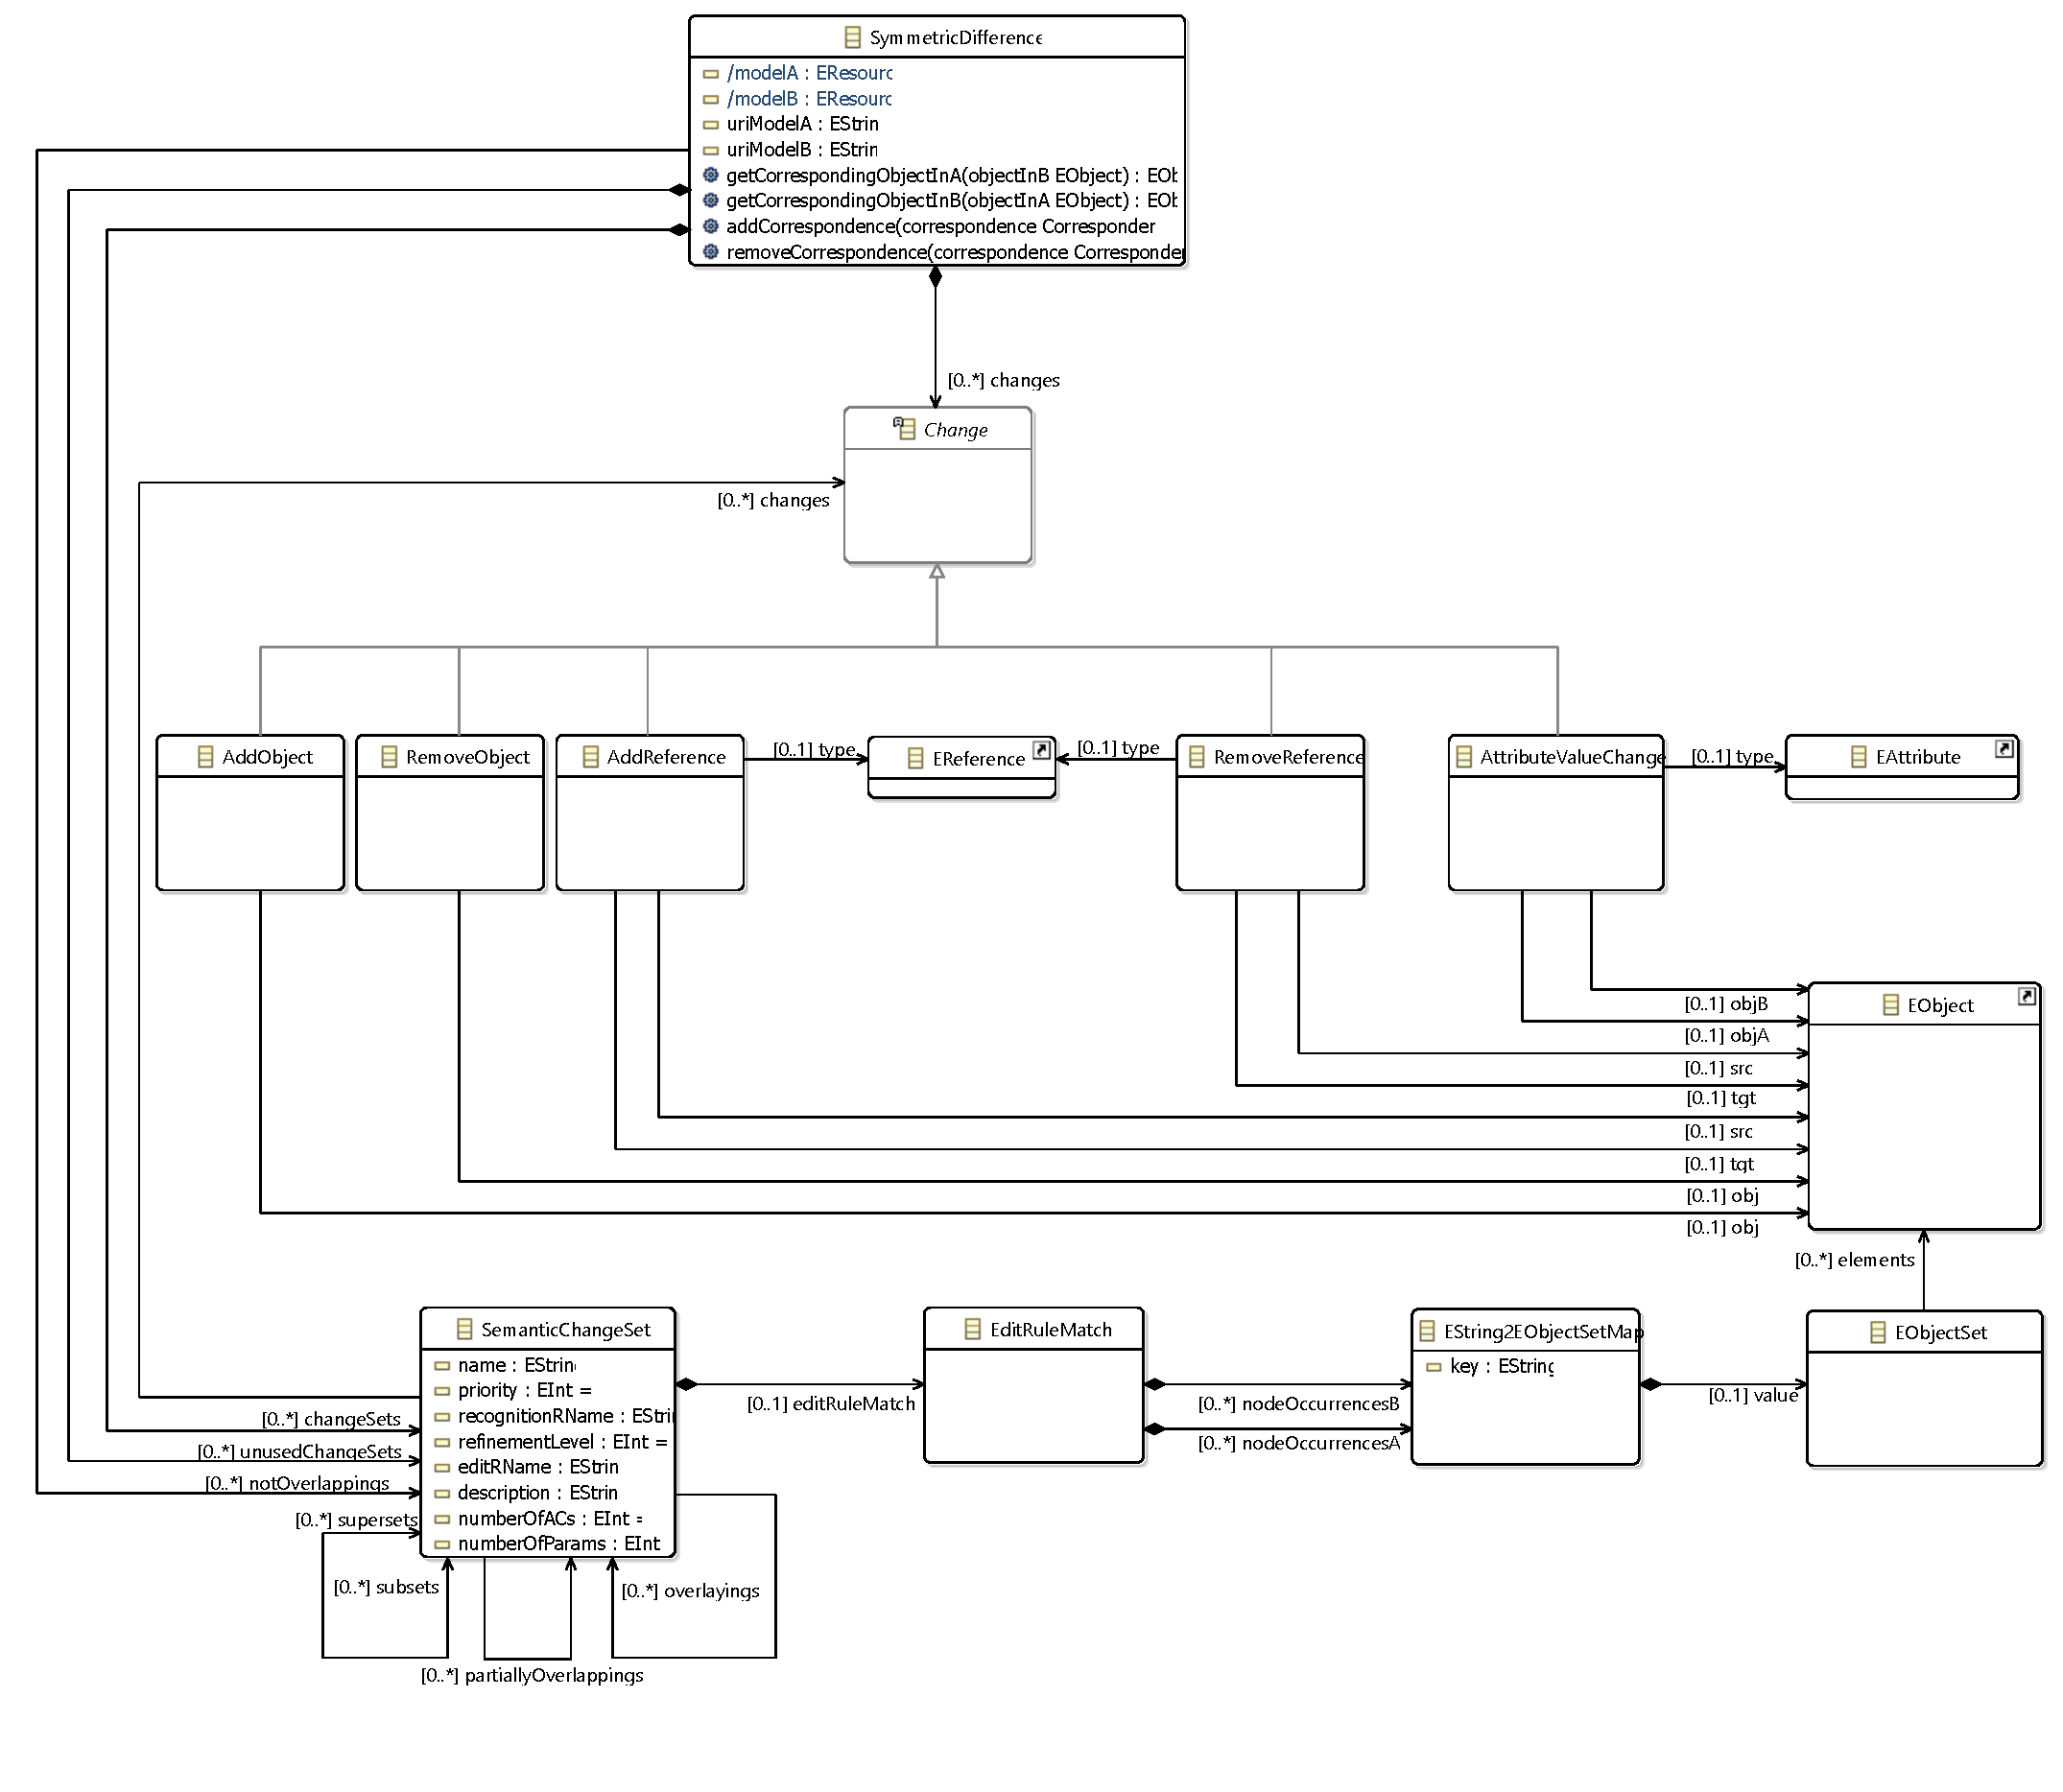
\includegraphics[width=\textwidth]{images/architecture/symmetric_model}
\caption{Abstract Syntax of a descriptive model difference}
\label{fig:symmetric_model}
\end{figure}

\begin{figure}[h!]
\centering
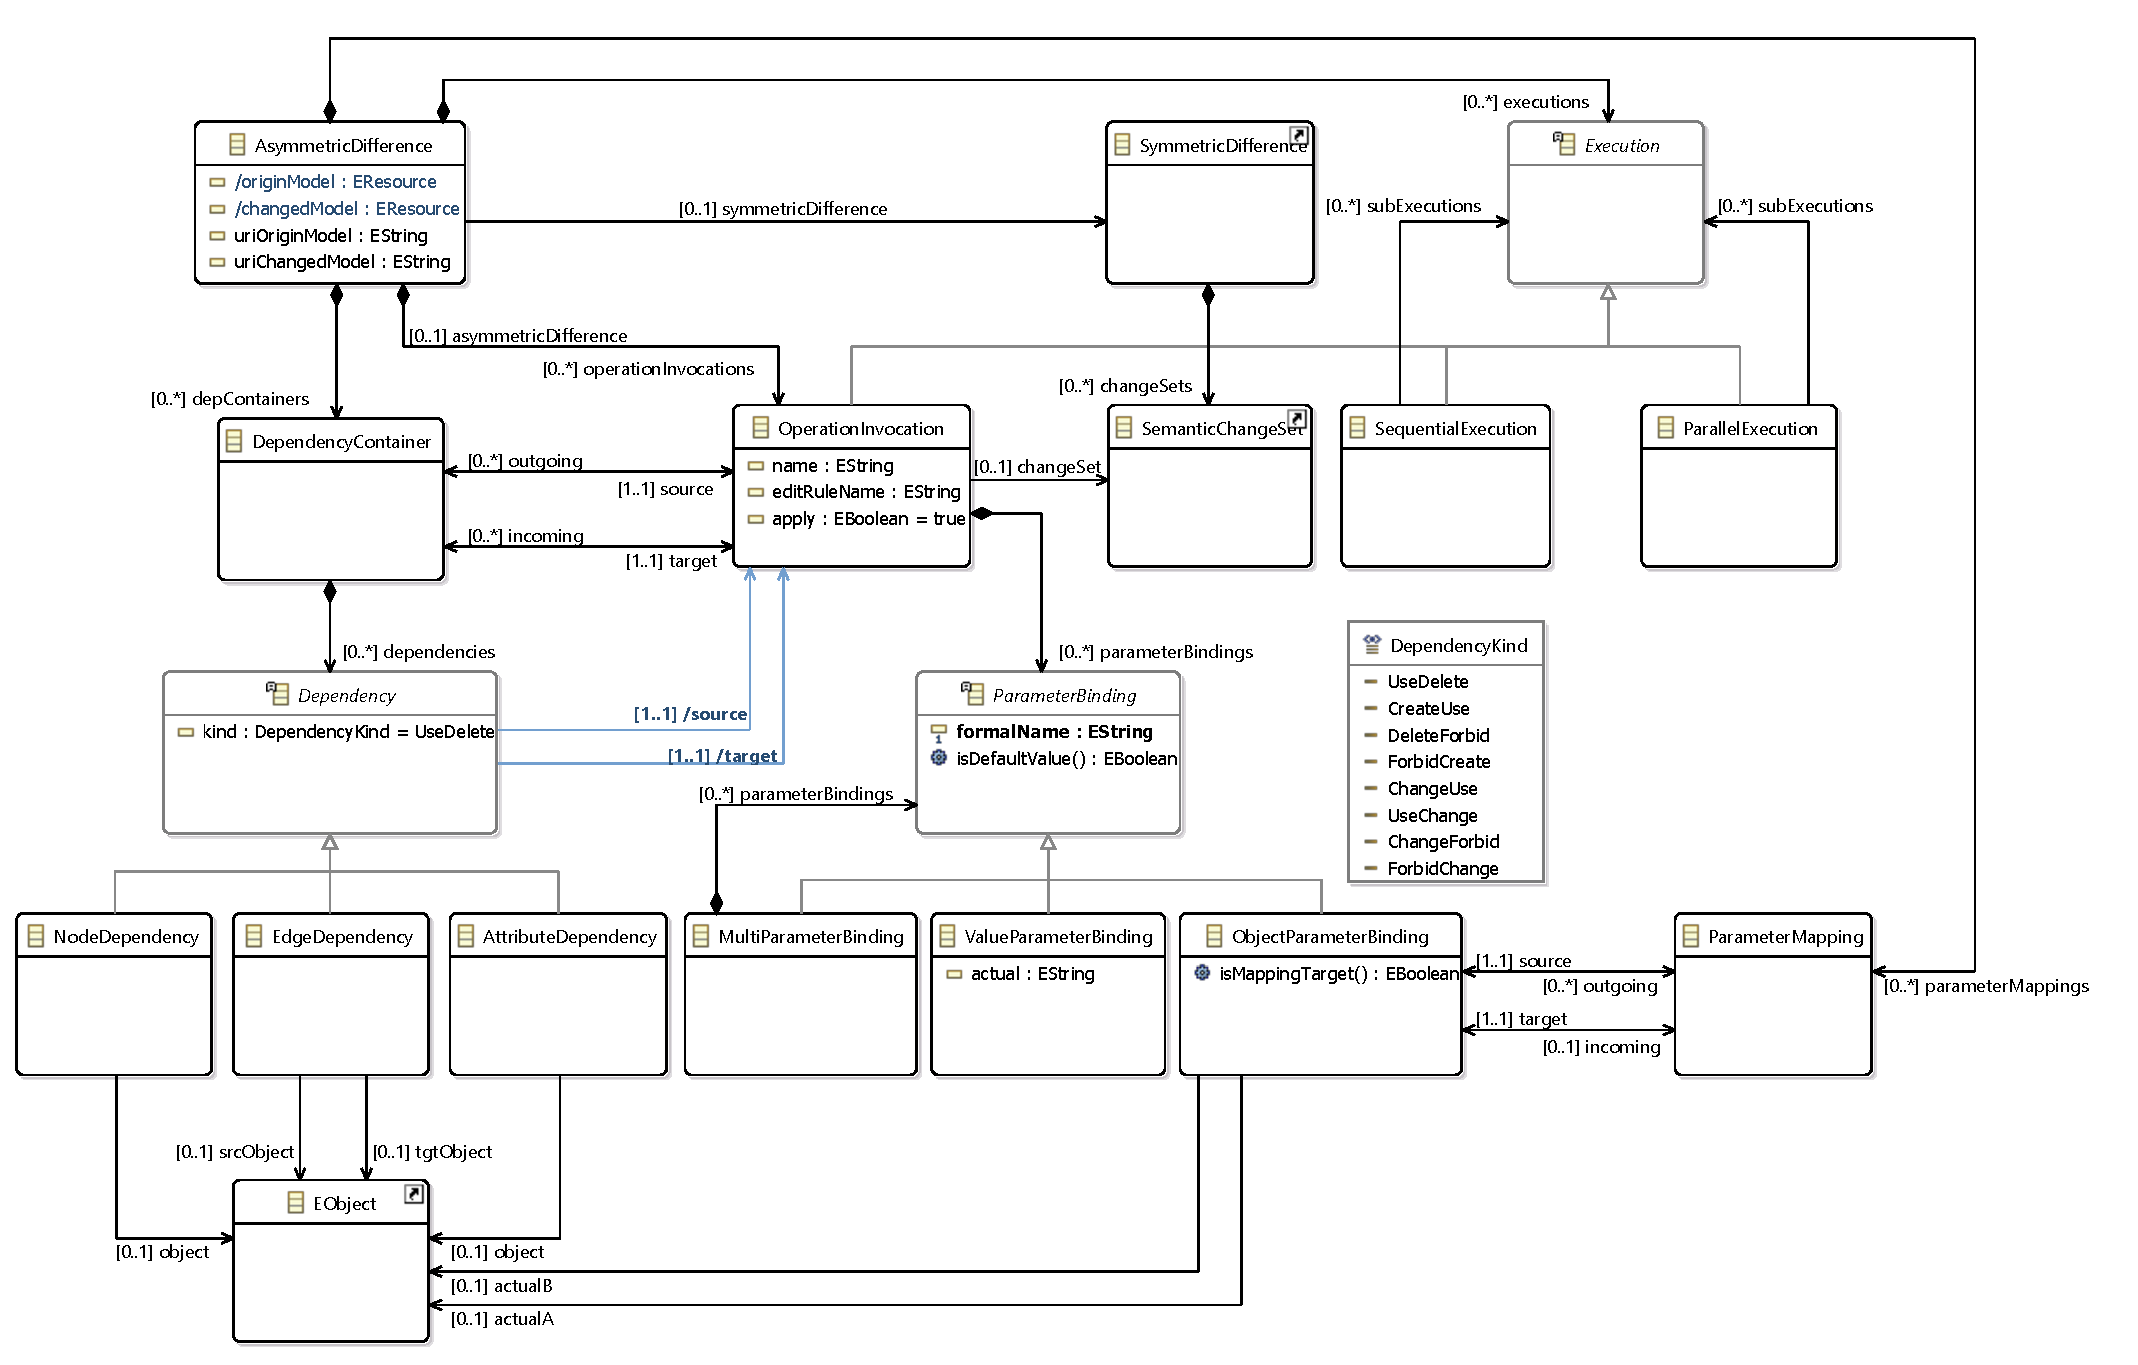
\includegraphics[width=\textwidth]{images/architecture/asymmetric_model}
\caption{Abstract Syntax of a prescriptive model difference}
\end{figure}

\newpage


\subsection{Rule Base}

\begin{figure}[h!]
\centering
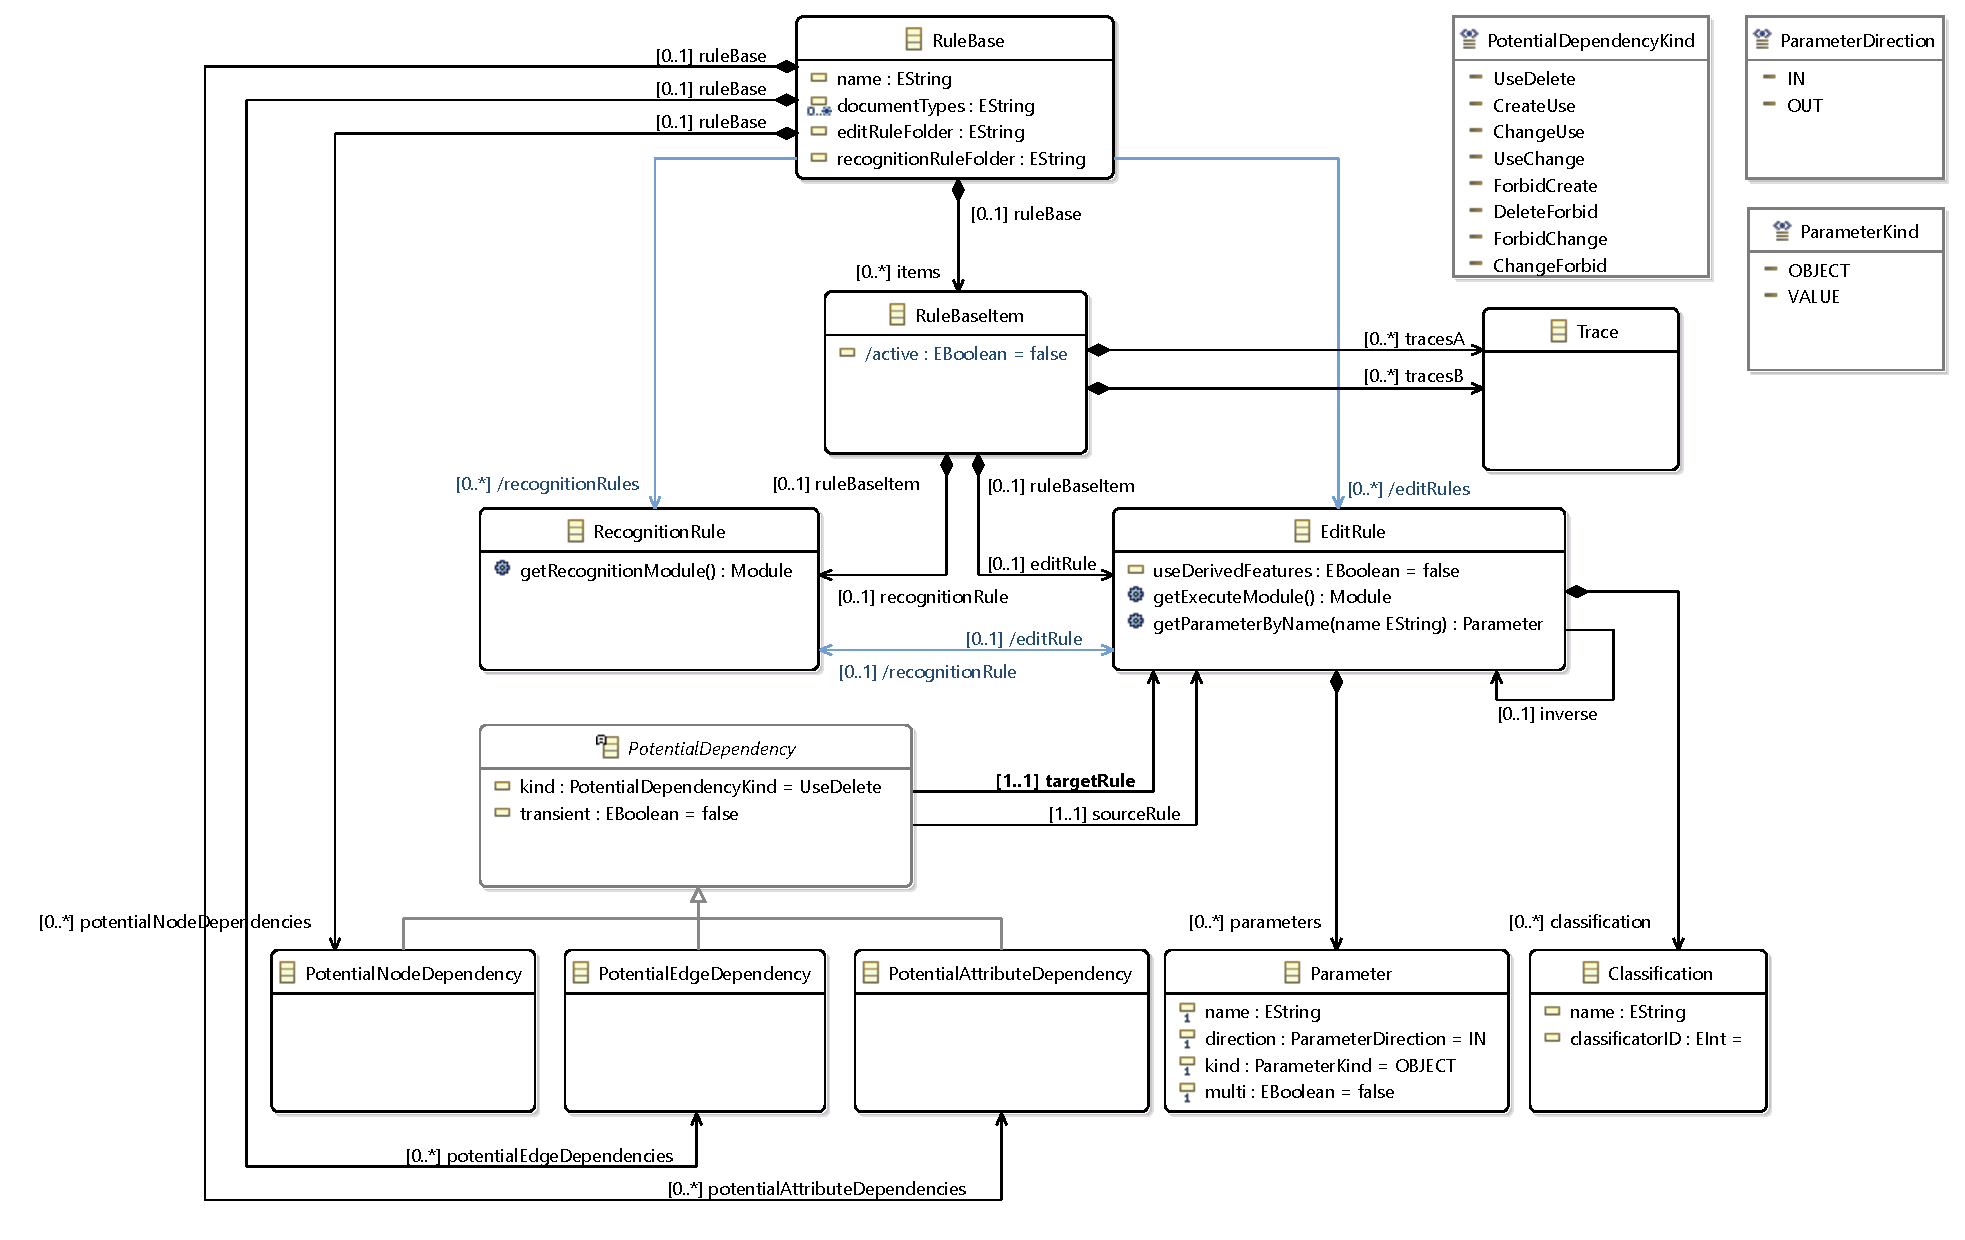
\includegraphics[width=\textwidth]{images/architecture/rulebase_model}
\caption{Conceptual structure of a rule base}
\end{figure}


